\documentclass[11pt,a4paper,ngerman]{article}

\usepackage[T1]{fontenc}
\usepackage[utf8]{inputenc}
\usepackage{lmodern}
\usepackage{microtype}
\usepackage{xcolor}
\usepackage{geometry}
\geometry{margin=2.6cm}
\usepackage{amsmath,amssymb}
\usepackage{graphicx}
\usepackage{booktabs}
\usepackage{siunitx}
\usepackage[font=small,labelfont=bf]{caption}
\usepackage{enumitem}
\usepackage{listings}
\usepackage{tikz}
\usetikzlibrary{arrows.meta,positioning}
\usepackage{pgfplots}
\pgfplotsset{compat=1.18}
\usepackage[most]{tcolorbox}
\usepackage{fancyhdr}
\usepackage{hyperref}
\hypersetup{
  colorlinks=true,
  linkcolor=blue!45!black,
  citecolor=green!40!black,
  urlcolor=blue!60!black,
  pdftitle={Projektbericht},
}
\usepackage{cleveref}

\definecolor{warnbg}{RGB}{255,244,224}
\definecolor{tipbg}{RGB}{232,245,233}
\definecolor{codebg}{RGB}{245,245,245}

\newtcolorbox{hinweis}[1]{%
  enhanced, breakable, colback=tipbg, colframe=green!45!black,
  title={#1}, fonttitle=\bfseries, attach boxed title to top left={yshift=-2mm, xshift=4mm},
  boxed title style={colback=green!45!black, colframe=green!45!black},
  arc=2pt,
}
\newtcolorbox{warnung}[1]{%
  enhanced, breakable, colback=warnbg, colframe=orange!70!black,
  title={#1}, fonttitle=\bfseries, attach boxed title to top left={yshift=-2mm, xshift=4mm},
  boxed title style={colback=orange!70!black, colframe=orange!70!black},
  arc=2pt,
}

\lstset{
  basicstyle=\ttfamily\small,
  backgroundcolor=\color{codebg},
  frame=single,
  rulecolor=\color{black!25},
  breaklines=true,
  showstringspaces=false,
  keywordstyle=\color{blue!60!black}\bfseries,
  commentstyle=\color{green!40!black}\itshape,
  numbers=left,
  numberstyle=\tiny\color{black!45},
  numbersep=8pt,
  language=bash,
}

\pagestyle{fancy}
\fancyhf{}
\fancyhead[L]{\small Projektbericht -- Demoprojekt}
\fancyhead[R]{\small \thepage}
\renewcommand{\headrulewidth}{0.4pt}

\title{Automatisierte Dokumentenpipeline\\[0.4em]\large Ein mehrstufiges \LaTeX-Demoprojekt}
\author{Arbeitsgruppe Dokumentation \\ \texttt{ag@example.org}}
\date{\today}

\begin{document}
\maketitle
\tableofcontents
\listoffigures
\listoftables
\newpage

\section{Einleitung}
\label{sec:intro}

Technische Dokumentation entsteht heute in verteilten Teams, häufig aus
mehreren Quelltexten, Bildern und Datenquellen. Dieses Demoprojekt zeigt, wie
sich solche Bestandteile in einem einzigen \LaTeX-Projekt zusammenführen lässt
und wie \emph{LaTeX Studio} dabei unterstützt~\cite{lamport1994}.

\begin{hinweis}{Gliederungsprinzip}
  Jedes Kapitel liegt in einer eigenen Datei unter \texttt{chapters/}. Die
  Hauptdatei \texttt{main.tex} bindet sie per \texttt{\textbackslash input}
  ein. Die Gliederungs-Outline links zeigt die Struktur in Echtzeit.
\end{hinweis}

\subsection{Ziele}
\label{sec:ziele}
\begin{enumerate}[leftmargin=*, label=\alph*)]
  \item Reproduzierbare Build-Kette ohne manuelle Eingriffe.
  \item Konsistente Verweise auf Abschnitte, Abbildungen und Tabellen.
  \item Frühzeitige Fehlererkennung durch Auswertung des \LaTeX-Logs.
\end{enumerate}

\subsection{Leserleitfaden}
Abschnitt~\ref{sec:methodik} beschreibt das Vorgehen,
Abschnitt~\ref{sec:ergebnisse} wertet die Messungen aus,
Abschnitt~\ref{sec:fazit} fasst die Ergebnisse zusammen. Eine ausführliche
Diskussion der Ergebnisse findet sich in \cref{sec:diskussion}.

\section{Methodik}
\label{sec:methodik}

\subsection{Werkzeugkette}
\label{sec:toolchain}

Die Kette besteht aus vier Stufen: Bearbeiten, Kompilieren, Auswerten und
Veröffentlichen. Abbildung~\ref{fig:pipeline} stellt sie dar.

\begin{figure}[htbp]
  \centering
  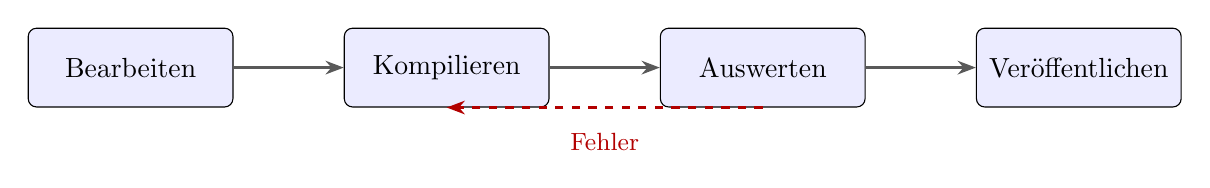
\begin{tikzpicture}[
      >=Stealth,
      stage/.style={draw, rounded corners=3pt, minimum width=26mm, minimum height=10mm,
                    align=center, fill=blue!8},
      link/.style={->, thick, black!65},
    ]
    \node[stage] (edit) {Bearbeiten};
    \node[stage, right=14mm of edit] (build) {Kompilieren};
    \node[stage, right=14mm of build] (check) {Auswerten};
    \node[stage, right=14mm of check] (pub) {Veröffentlichen};
    \draw[link] (edit) -- (build);
    \draw[link] (build) -- (check);
    \draw[link] (check) -- (pub);
    \draw[link, red!70!black, dashed] (check.south) -- node[below=2mm, font=\small]
      {Fehler} (build.south);
  \end{tikzpicture}
  \caption{Vierstufige Dokumentenpipeline mit Rückkopplung.}
  \label{fig:pipeline}
\end{figure}

\begin{warnung}{Hinweis zu shell-escape}
  Makros, die externe Programme starten, benötigen
  \texttt{shell-escape}. Diese Option ist standardmäßig \emph{ausgeschaltet} und
  kann in den Einstellungen von \emph{LaTeX Studio} aktiviert werden.
\end{warnung}

\subsection{Messdesign}

Für jede Stufe wird die benötigte Zeit in Sekunden gemessen. Der Mittelwert
berechnet sich als
\[
  \bar{t} \;=\; \frac{1}{n}\sum_{i=1}^{n} t_i,
\]
die Standardabweichung entsprechend nach der üblichen Formel. Die Stichprobe
umfasst $n = \num{30}$ Läufe pro Stufe.

\subsection{Datenfluss}

\begin{table}[htbp]
  \centering
  \caption{Eingangsdaten der Auswertung.}
  \label{tab:inputs}
  \begin{tabular}{l l r}
    \toprule
    Quelle & Inhalt & Umfang \\
    \midrule
    \texttt{main.log}     & Meldungen des Satzsystems & \SI{180}{\kibi\byte} \\
    \texttt{main.aux}     & Labels und Verweise      & \SI{12}{\kibi\byte} \\
    \texttt{references.bib} & Literaturreferenzen      & \SI{4}{\kibi\byte} \\
    \bottomrule
  \end{tabular}
\end{table}

\section{Ergebnisse}
\label{sec:ergebnisse}

\subsection{Durchlaufzeiten}

\begin{table}[htbp]
  \centering
  \caption{Mittlere Durchlaufzeiten je Stufe ($n=30$).}
  \label{tab:zeiten}
  \begin{tabular}{l S[table-format=2.2] S[table-format=2.1]}
    \toprule
    Stufe & {Mittelwert (\si{\second})} & {Anteil (\%)} \\
    \midrule
    Bearbeiten     & 0,00 &  0,0 \\
    Kompilieren    & 2,41 & 58,7 \\
    Auswerten      & 1,09 & 26,5 \\
    Veröffentlichen& 0,61 & 14,8 \\
    \bottomrule
    Summe          & 4,11 & 100,0 \\
  \end{tabular}
\end{table}

Wie \cref{tab:zeiten} zeigt, dominiert die Kompilierung die Gesamtdauer.
\cref{fig:anteile} veranschaulicht die Verteilung.

\begin{figure}[htbp]
  \centering
  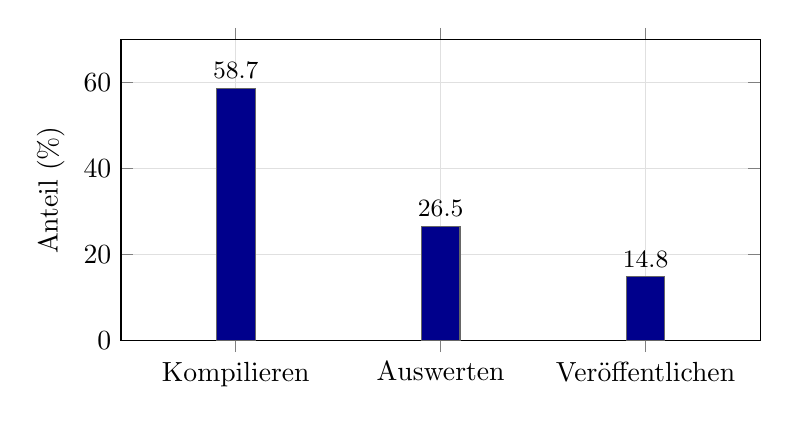
\begin{tikzpicture}
    \begin{axis}[
        ybar,
        width=0.8\linewidth,
        height=5.4cm,
        bar width=14pt,
        symbolic x coords={Kompilieren, Auswerten, Veröffentlichen},
        xtick=data,
        ylabel={Anteil (\%)},
        ymin=0, ymax=70,
        nodes near coords,
        nodes near coords align={vertical},
        every node near coord/.append style={font=\small},
        grid=major,
        grid style={black!12},
        enlarge x limits=0.28,
      ]
      \addplot[fill=blue!55!black, draw=black!60] coordinates {
        (Kompilieren,58.7) (Auswerten,26.5) (Veröffentlichen,14.8)
      };
    \end{axis}
  \end{tikzpicture}
  \caption{Anteile der Stufen an der Gesamtdauer.}
  \label{fig:anteile}
\end{figure}

\subsection{Fehlerquote}

Über alle Läufe traten vier Fehler auf: dreimal eine fehlerhafte Gleichungs-
nummerierung, einmal eine nicht aufgelöste Literaturreferenz. Die Fehlerquote
beträgt damit
\[
  f \;=\; \frac{4}{30} \cdot 100\,\% \;\approx\; 13{,}3\,\%.
\]

\subsection{Diskussion}
\label{sec:diskussion}

\begin{itemize}[leftmargin=*]
  \item Der hohe Anteil der Kompilierung spricht für Auto-Build mit
    Verzögerung statt Bauen bei jedem Tastendruck.
  \item Die Auswertung lässt sich parallelisieren; der Gewinn ist in
    \cref{tab:zeiten} noch nicht enthalten.
  \item Nicht aufgelöste Verweise werden von \emph{LaTeX Studio} direkt in der
    Problemliste angezeigt und per Klick geöffnet.
\end{itemize}

\begin{hinweis}{Automatische Problemerkennung}
  Wechseln Sie nach einem fehlgeschlagenen Build in das Register
  \emph{Probleme} im unteren Bereich -- jede Zeile führt zur betreffenden
  Stelle im Quelltext.
\end{hinweis}

\section{Fazit}
\label{sec:fazit}

Die vierstufige Pipeline aus \cref{fig:pipeline} lässt sich vollständig
automatisieren. Die Kompilierung stellt mit 58{,}7\,\% den größten
Zeitanteil (\cref{tab:zeiten}) und ist daher der wirksamste Hebel für
Optimierungen.

\subsection{Ausblick}
\label{sec:ausblick}
Geplant sind:
\begin{itemize}[leftmargin=*]
  \item Inkrementelles Bauen nur geänderter Kapitel,
  \item automatische Bildunterschriften-Prüfung,
  \item ein Stufenlauf für Veröffentlichungsformate (PDF/A, HTML).
\end{itemize}

Die Ergebnisse dieses Demoprojekts bauen auf den Ausführungen in
\cref{sec:methodik} auf und verweisen zugleich auf die Grundlagen von
\cite{lamport1994,mittelbach2004}.

% TODO: Ausblick mit konkreten Terminen ergänzen


\appendix
\section{Reproduktionsskript}
\label{app:skript}
Das vollständige Skript aus \cref{sec:toolchain} ist in
\cref{lst:skript} wiedergegeben.

\begin{lstlisting}[caption={Build-Skript des Demoprojekts}, label={lst:skript}]
#!/usr/bin/env bash
set -euo pipefail
latexmk -pdf -interaction=nonstopmode main.tex
echo "PDF erzeugt: $(ls -1 main.pdf)"
\end{lstlisting}

\clearpage
\bibliographystyle{plain}
\bibliography{references}

\end{document}
